% fs setup
\PassOptionsToPackage{pdfpagelabels=false}{hyperref}
% \documentclass[useAMS,fleqn,usenatbib]{mnras} % fleqn left-aligns equations
\documentclass[useAMS,usenatbib]{mnras}
\pdfoutput=1 %for arxiv
\setlength{\topmargin}{-0.3in}

\usepackage{graphicx}
\usepackage{amsmath,amssymb,amstext}
\usepackage[T1]{fontenc}
\usepackage{ae,aecompl}
\usepackage[utf8]{inputenc}
% \usepackage{newtxtext,newtxmath}
\usepackage[figure,figure*]{hypcap}
\usepackage[dvipsnames]{xcolor}
\usepackage{bm}

\usepackage{xparse}

%% MINE
\usepackage{xspace} % smart spaces after custom \newcommand



%----------------------------------------
\newcommand{\qus}[1]{{\color{BrickRed}\textbf{[Q: }\textbf{#1}]}}
\newcommand{\arz}[1]{{\color{ForestGreen}\textbf{[Andrew: }\textbf{#1}]}}
\newcommand{\jan}[0]{{\color{TealBlue}\textbf{[Jeff: ]}}}
\newcommand{\tjr}[1]{{\color{Brown}\textbf{[Troy: }\textbf{#1}]}}


%-- Units
\newcommand{\Msun}{\mathrm{M}_{\odot}} % Msun
\newcommand{\Mstar}{\mathrm{M}_{\star}} % Mstar
\newcommand{\Msunh}{h^{-1}\mathrm{M}_{\odot}} % Msun/h
\newcommand{\hmpc}{\mathrm{h}^{-1}\mathrm{Mpc}} % Mpc/h
\newcommand{\kms}{\mathrm{km/s}}
\newcommand{\gev}{\mathrm{GeV}}

%-- Words
\newcommand{\lcdm}{$\Lambda$CDM\xspace}
\newcommand{\photoz}{photo-$z$\xspace}
\newcommand{\photozs}{photo-$z$'s\xspace}
\newcommand{\Photozs}{Photo-$z$'s\xspace}
\newcommand{\specz}{spec-$z$\xspace}
\newcommand{\speczs}{spec-$z$'s\xspace}
\newcommand{\z}{$z$\xspace}
\newcommand{\Z}{$Z$\xspace}


%-- Code packages
\newcommand{\mesa}{\texttt{MESA}\xspace}
\newcommand{\fortran}{\texttt{Fortran}\xspace}
\newcommand{\python}{\texttt{Python}\xspace}
\newcommand{\rockstar}{\texttt{ROCKSTAR}\xspace}
\newcommand{\halotools}{\texttt{Halotools}\xspace}
\newcommand{\corrfunc}{\texttt{Corrfunc}\xspace}
\newcommand{\glue}{Glue\xspace}
\newcommand{\xgboost}{\texttt{XGBoost}\xspace}
\newcommand{\gpz}{\texttt{GPz}\xspace}




%-- Figures and Equations
\newcommand{\equ}[1]{\[#1\]}
\newcommand{\nequ}[2]{\begin{equation}#1 \label{#2}\end{equation}}
\newcommand{\equin}[1]{\(#1\)}
\newcommand{\figscale}[4]{
% commands: width scale, path, caption, label
\begin{figure}[h]
    \centering
    \includegraphics[width=#1\textwidth]{#2}
    \caption{#3}
    \label{#4}
\end{figure}
}


\usepackage{url}

%% ENDMINE

%%%%%%%%%%%%%%%%%%% TITLE PAGE %%%%%%%%%%%%%%%%%%%

% Title of the paper, and the short title which is used in the headers.
% Keep the title short and informative.
\title[Asymmetric Dark Matter in Stars]{The Effects of Asymmetric Dark Matter on Stellar Evolution I: Spin-Dependent Scattering}

% The list of authors, and the short list which is used in the headers.
% If you need two or more lines of authors, add an extra line using \newauthor
\author[T.J. Raen et al.]{%
Troy J. Raen,$^{1}$\thanks{E-mail: troy.raen@pitt.edu},
Héctor Martínez-Rodríguez$^{1}$,
Andrew R. Zentner$^{1}$,
Travis J. Hurst$^{2}$, \newauthor
Carles Badenes$^{1}$,
and Rachel Tao$^{3}$
\vspace*{12pt}
\\
% List of institutions
$^{1}$Department of Physics and Astronomy \& Pittsburgh Particle Physics, Astrophysics, and Cosmology Center (Pitt PACC),\\ University of Pittsburgh, Pittsburgh, PA 15260, USA\\
$^{2}$Department of Mathematics and Physics, Colorado State University -  Pueblo, Pueblo, C0, 81001 \\%Fixed my contact info. TJH
$^{3}$Department of Physics, Emory University, Atlanta, GA 30322
}
% These dates will be filled out by the publisher
\date{\today}

% Enter the current year, for the copyright statements etc.
\pubyear{2019}

% Don't change these lines
\begin{document}
\label{firstpage}
\pagerange{\pageref{firstpage}--\pageref{lastpage}}
\maketitle

% fe setup

% Abstract of the paper
\begin{abstract}
We study the effects of Dark Matter on the evolution of stars with masses 0.8-5.0$\Msun$ and find that, in certain environments, main sequence lifetimes can be dramatically altered. \tjr{Finish writing abstract...}
\end{abstract}

% Select between one and six entries from the list of approved keywords.
% Don't make up new ones.
\begin{keywords}
keyword1 -- keyword2 -- keyword3
\end{keywords}

%%%%%%%%%%%%%%%%%%%%%%%%%%%%%%%%%%%%%%%%%%%%%%%%%%







%%%%%%%%%%%%%%%%% BODY OF PAPER %%%%%%%%%%%%%%%%%%

\todo{find other stellar textbook(s) to cite.}


\vspace{10mm}

\section{Introduction}
\label{sec:intro}

  \arz{Upon reading this, I think I prefer not to abbreviate dark matter,
  but you can make the final decision.}

  % \arz{I think I like $\mdm$ for the dark matter particle mass. The
  % problem with using $\chi$ is that it is heavily tied to the WIMP scenario because
  % in the case of a SUSY WIMP, $\chi$ is the symbol for the neutralino that might
  % be the dark matter. Thus, using $\chi$ suggests that SUSY WIMP scenario, which
  % we don't want to do.}

  \arz{I added a number of references to "bib.bib." For some reason, I couldn't
  open "references.bib."}

  A preponderance of the evidence suggests that approximately $84\%$ of the matter budget of the
  universe consists of a form of non-baryonic dark matter that has yet to be identified.
  \arz{Let's cite a few dark matter review articles here including Jungman+96, Bertone+2006, the
  Cosmic Visions report. Let's also cite some of the standard references for constraints on
  cosmological parameters, such as the Planck result.} In
  the standard picture of cosmological structure formation,
  galaxies form within the potential wells of
  large, nearly virialized halos of dark matter \citep{white_rees78,blumenthal_etal84}.
  If the dark matter interacts with standard model particles,
  it can be captured by stars moving through dark matter halos
  \citep{press_spergel85,krauss_etal85, gaisser_etal86, griest_seckel87}.
  Once captured, continued scattering within the stellar interior contributes
  to energy transport within the star, potentially altering its evolution \citep{Spergel1985EffectInterior, Zentner2011AsymmetricDwarfs}
  \tjr{get a few more references} \arz{Good idea. Look for papers by Fabio Iocco,
  Ian Shoemaker, Malcolm Fairbairn, Jordi Casanellas, Ilidio Lopez}.
  The significance of this energy transport depends on the following
  properties (in addition to the properties of the star):
  (1) the dark matter mass, $\mx$;
  (2) the dark matter-nucleon scattering cross section, $\sigxn$;
  and (3) the total number of dark matter particles captured by a star, $\Nx$,
  which itself depends on $\sigxn$ as well as the local dark matter environment from
  which the particles are captured (see \S~\ref{sec:props}).
  We study the effects of energy transport by asymmetric dark matter
  (ADM, see below)
  in stars of mass \mrange living within a variety of dark matter
  environments, using the publicly available code
  Modules for Experiments in Stellar Astrophysics \citep[\mesa,][]{Paxton2011ModulesMESA}.

  Evidence supporting the claim that $\sim$84\% of the matter in the universe is in
  an unknown form of dark matter is abundant and varied, ranging from the
  anisotropy of the microwave background radiation to formation and structures of galaxies.
  \arz{cite reviews here.}
  However, dark matter has only been observed indirectly, through its
  gravitational influence, and much remains to be discovered about its fundamental nature.
  For several decades, the leading candidate has been the so called Weakly-interacting massive particle (WIMP).
  The classic WIMP is a heavy ($\mx \sim 10^2-10^3 \gev$) thermal relic whose contemporary abundance is set
  by its annihilation rate in the early universe \arz{cite e.g., Kolb and Turner textbook
  or some other standard reference for the reader that needs a definition of a thermal relic}.
  Therefore, WIMPs are thought to have a fairly well established ``standard'' annihilation
  cross section \citep[e.g.,][]{steigman_etal12}. This annihilation, in turn, limits the number of particles
  that can accumulate within a star as the rate of capture of new dark matter particles
  equilibrates with annihilation in the stellar interior \citep{krauss_etal85}.
  Despite numerous, ongoing terrestrial direct detection experiments \arz{cite LUX, CRESST,
  and so on. maybe ask Brian Batell for references to the very latest results here.} and
  efforts to detect dark matter indirectly through its annihilation products \arz{cite the FERMI, HESS,
  and VERITAS results here as well as IceCube constraints on dark matter},
  dark matter has not been observed non-gravitationally. The
  available parameter space for classic WIMPs is rapidly shrinking
  \citep{Amole16} \tjr{Still need to refer to a constraint paper.},
  which has triggered a surge in research into alternatives to the long-favored WIMP.


  Asymmetric dark matter (ADM) is an alternative to the classic WIMP in which
  the relic abundance of the dark matter particle is set by a primordial asymmetry
  rather than via annihilation \citep[for a review, see][and references therein]{adm_review}.
  If the baryon and dark matter asymmetries are
  related, then such models have the appealing property that they explain
  the fact that the contemporary dark matter and baryon abundances are
  of the same order of magnitude, which is otherwise surprising because
  these relic abundances are determined by unrelated physics in the WIMP
  scenario. The variety of specific incarnations of ADM is broad,
  but ADM models typically predict particle masses smaller than
  the classic WIMP ($\mx \sim 1-10 \gev$) and no contemporary
  dark matter annihilation due to the present-day absence of
  dark matter anti-particles.


  These predictions motivate studies to
  constrain ADM indirectly through stellar astrophysics. The lack of
  annihilation means that ADM may build up to very large
  quantities within stars because the capture of ADM is never countered
  by annihilation. Meanwhile, the relatively low masses
  compared to the classic WIMP mean captured ADM particles orbit within
  a significant volume of the star, out to $r_{\mathrm{DM}} \sim X$ \arz{Put number here.}
  for a Sun-like star, which means that they experience large differences
  in ambient temperature
  throughout their orbits and can thus transport energy outward from the
  stellar core extremely efficiently \citep{Spergel1985EffectInterior}.
  These features of ADM have already motivated research into the possibility that
  ADM may alter stellar evolution
  \citep[e.g.][]{Zentner2011AsymmetricDwarfs,iocco_etal12,vincent_etal15}.
  In this paper we undertake a study of the properties and evolution of
  stellar populations within halos of ADM. In this first paper on the topic,
  we further narrow our study to spin-dependent ADM-nucleus scattering.
  In contrast, spin-independent ADM-nucleus scattering leads to behaviors that are
  qualitatively distinct; therefore we will
  present results for this case in a forthcoming manuscript.

  % \arz{How about this edit (starting with a new paragraph)?}
  %   The degree of stellar cooling induced by dark matter
  %   depends upon the following DM properties:
  %   1) the WIMP mass $m_x$;
  %   2) the WIMP-nucleon scattering cross section $\sigma_{xn}$;
  %   and 3) the total number of WIMPs captured by a star $N_x$.
  %   We will characterize stellar cooling using these parameters.
  %   As we will show below, our results are most relevant to a class
  %   of dark matter models known as {\em asymmetric dark matter} (ADM)
  %   \arz{Need some generic ADM citations here, start by looking in my paper.}
  %   The number of standard WIMP dark matter particles that can be captured
  %   within a star is limited by the fact that WIMP capture will come to
  %   equilibrium with WIMP mutual annihilation within the star. In ADM models,
  %   the dark matter does not annihilate because the dark matter consists entirely
  %   of dark matter particles and is completely devoid of dark matter antiparticles.
  %   For this reason, $N_x$ can grow very large in ADM models, enabling the
  %   effects of dark matter on stellar evolution to grow correspondingly large
  %   over the lifetime of a star. Consequently, our proposal is to use
  %   astrophysical studies of stellar populations to constrain ADM. In this first
  %   paper, we further narrow our study to spin-dependent ADM-nucleus scattering
  %   because spin-dependent and spin-independent scattering lead to qualitatively
  %   distinct behaviors. We will present results for spin-independent scattering
  %   in a forthcoming manuscript.

  We generally find that ADM captured by stars can cool stellar cores to a degree that can have potentially
  observable effects on stellar populations. In general, the extra cooling due to ADM reduces the MS lifetimes \tjr{since the intro to stellar models got moved down, the MS hasn't been introduced yet...}
  of stars and alters their subsequent evolution \qus{this last part doesn't make sense to me. The stars cross the sub-giant branch at a lower luminosity but after that the evolution is the same.}. We summarize our results on stellar lifetimes in Figure~\ref{fig:mstau}
  and the net effect on stellar populations in the form of stellar isochrones in Figure~\ref{fig:isos_cb} in
  \S~\ref{sec:results}. The effects of stellar cooling are particularly large in environments in which
  the ambient dark matter density is high and velocity dispersion is low, such that the capture of
  dark matter is extremely efficient. Thus, these effects will be largest in dwarf satellite galaxies
  and high-redshift galaxies.

  In the following section, we summarize the dependence of the capture rate of dark matter
  within stars on dark matter and stellar properties. In \S~\ref{sec:methods}, we describe
  our simulations of stellar evolution including cooling due to ADM. We present our results
  in \S~\ref{sec:results}. We discuss our results and draw conclusions in \S~\ref{sec:conclusions}.


\arz{I commented out two paragraphs here. I don't think we need them.}
  \tjr{I'm a bit surprised that you think all of the 2nd paragraph is unnecessary.. I had guessed that this would not be common knowledge to someone who studies dark matter and not stars...?}
  %  We present our final results in the form of Hertzsprung–Russell (HR) diagrams\footnote{Note that an observer's HR diagram plots color versus magnitude while theorists use $\Teff$ and $L$ which captures the same information. \qus{do I need this footnote?}}. In Figure \ref{fig:tracks} we plot stellar tracks (properties are functions of time for a given stellar mass). In Figure \ref{fig:isos_cb} we plot isochrones (properties are functions of stellar mass for a given age).
  %
  %  The observed luminosity, $L$, and effective temperature, $\Teff$, of a MS star remain roughly constant over human time scales; however, these observables do vary as a function of mass, making star clusters feasible testing grounds for DM constraints. All stars in a cluster live in the same DM environment and are assumed to have formed from a single molecular cloud, meaning they have approximately the same age and metallicity. Given a stellar evolution model and an initial mass function for the cluster, its properties can be predicted and isochrones compared to observations. We leave quantitative constraints to future work since they will require in-depth analysis of stellar demographics \qus{and environments?}.
  %
  %
  %


% \subsection{Observing Stellar Evolution}
%
%   \tjr{Are there other parts of the paper for which this is also true?}
%   \arz{The information in this section is all correct and you should hang on to it
%   for the purposes of writing your thesis document, but... I would say that this
%   information is not necessary in a journal article. So, I would get rid of the
%   subsection heading and reduce this section to one, short paragraph.
%   I think that we can say that
%   we cast our final results into the form of H-R or color-magnitude diagrams and that
%   we defer taking this all the way to a constraint for a future paper. The reason for
%   deferring is simply that extracting an actual constraint from observational data
%   requires a great deal of work on stellar demographics that suffices to constitute a
%   publication of its own.}
%
%   Ultimately, the effects we calculate can be compared to observations to further constrain DM properties. We leave this comparison to future work, but will briefly describe the process in order to focus our results.
%
%   Stellar evolution is best observed using Hertzsprung–Russell (HR) diagrams\footnote{Note that an observer's HR diagram plots color versus magnitude while theorists use T$_{\rm{eff}}$ and L which captures the same information.} of star clusters. All stars in the cluster are assumed to have formed from a single molecular cloud and therefore to have approximately the same metallicity and age. For this reason these diagrams are also called isochrones. Given a stellar evolution model and an initial mass function for the cluster, their properties can be predicted and compared to observations.
%
%   Since the MS is a near equilibrium state, with gravitational contraction balanced by outward radiation pressure from nuclear burning, the observed luminosity, L, and effective temperature, T$_{\rm{eff}}$, remain roughly constant at values which increase with the star's total mass. Then MS stars lie roughly along a line with negative slope in an HR diagram (see Figure \ref{fig:stellarHR}).
%
%   As the core hydrogen supply depletes, the local burning rate must also decrease and the star leaves the MS. With less radiation pressure to counter gravity, the core contracts and the temperature rises. Once the temperature just outside the depleted core is sufficiently high, the hydrogen in that region ignites and the star enters a period of hydrogen shell burning. (This process happens quickly in  high mass stars and gradually in low mass stars, see Section \ref{sec:results} for details.) The shell burning region acts as a mirror and evolve up and to the right as they leave the MS \tjr{needs better explanation}. High mass stars have much higher central burning rates and so they burn through their hydrogen supply much more quickly. MS lifetimes are then inversely proportional to mass, and so a cluster's age can be determined by the location of this MS turn-off on the isochrone.
%
%   % %--------------------
%   % % stellar HR plots
%   % \begin{figure*}
%   % \centering
%   %   \includegraphics[width=\textwidth]
%   % %   {plots/HR_1_and_3p5_Msun.png}
%   % {plots/HR.png}
%   %   \caption{\label{fig:stellarHR}HR diagrams of the evolution of $1\Msun$ and $3.5\Msun$ stars. Only NoDM and c6 are shown for brevity. Marked positions correspond to the time the central hydrogen mass fraction falls below a threshold: ZAMS: 0.71, IAMS: 0.3, H-3: $10^-3$. (ZAMS and IAMS are used in Dotter.) Both models settle onto the MS at the same position in the HR plane, but move through the MS in different ways. NOTE: The data is cut: removed most of pre-MS and after MS turnoff. These cuts make it easier to see what I'm trying to show, but I'm not sure that my specific choices were the best. We should discuss.
%   %   }
%   % \end{figure*}
%   % %--------------------


%--------------
\section{Dark Matter Properties and Capture in Stars}
\label{sec:props}

  Probing the parameter space of ADM with simulations of stellar evolution is computationally expensive.
  Consequently, we show results for a representative set of ADM parameters chosen to:
  (1) make the effects of ADM on stellar evolution significant;
  and (2) remain consistent with contemporary constraints on dark matter properties.
  For our models we choose $\mx = 5 \gev\ (\approx 5m_p)$ and a spin-dependent
  scattering cross section of $\sigxp = 10^{-37} \cmsq$. \qus{I see that you took out the footnote explaining that the overwhelming majority of spin-dependent DM scattering events in MS stars are with protons. Is that so obvious that it doesn't need to be stated?} We assume that ADM self-interactions
  are negligible throughout; however, it is likely that self-interactions would lead to enhanced
  cooling \citep[e.g.,][]{Zentner2009High-energySun} and exploring such models would
  constitute a potentially interesting follow-up to this work.


  \tjr{Need something here on current m$_x$ and $\sigma_x$ constraints.}
  \arz{Yes, we need something here. It should just be a sentence saying that
  these parameters are just below the contemporary constraints on spin-dependent
  dark matter-nucleon scattering and give a citation to the latest result.
  I'm guessing you got this from Brian already, but the Cosmic Visions report
  from last year gives a nice summary along with links to all of the relevant
  experiments.}

  The energy transported by dark matter is proportional to the amount of ADM within the star.
  In ADM models, in which annihilation of dark matter within the star is negligible, the number
  of dark matter particles within the star at time, $t$, is given by $\Nx = \Cx t$
  where $\Cx$ is the capture rate. We use the capture rate from \citet{Zentner2011AsymmetricDwarfs},
  which is a simplified form valid for dark matter particle masses
  $\mx \lesssim 20 \gev$ \citep[see][ for more complete capture rates]{Gould1992CosmologicalAnnihilations,Zentner2009High-energySun}:
  %
  \begin{align}
  \begin{split}
    \label{eq:capturerate}
    \Cx =\ & \Csun
    \Big(\frac{\rhox}{0.4 \gev \cmcinv}\Big)
    \Big(\frac{270 \kms}{\bar{v}}\Big) \\
    & \times \Big(\frac{\sigxp}{10^{-43} \cmsq}\Big) \Big(\frac{5 \gev}{\mx}\Big) \\
    & \times \Big(\frac{v_{\mathrm{esc}}}{618 \kms}\Big)^2
    \Big(\frac{\Mstar}{\Msun}\Big)
  \end{split}
  \end{align}
  %
  where $\Csun = 5 \times 10^{21} \sinv$,
  $\rhox$ is the DM density in the stellar environment,
  $\bar{v}$ is the velocity dispersion of dark matter particles
  in the stellar neighborhood, and $v_{\mathrm{esc}}$ is the escape speed from the
  surface of the star.
  % This capture rate depends on both the properties of the ADM and the dark matter halo in which the star lives.

  The first line of Eq.~(\ref{eq:capturerate}) gives the dependence of the capture rate on stellar environment.
  Both $\rhox$ and $\bar{v}$ are properties of the local stellar environment. Moreover,
  these properties are degenerate with one another in Eq.~(\ref{eq:capturerate}); a higher ambient density
  of dark matter leads to a higher rate of capture, while a lower relative velocity between
  the star and the infalling dark matter leads to a higher probability for capture. Therefore it is convenient to parameterize a star's local dark matter
  environment by an overall factor \citep{Zentner2011AsymmetricDwarfs,Hurst2015},
  %
  \begin{equation}
  \gb = \Big(\frac{\rhox}{0.4 \gev \cmcinv}\Big) \Big(\frac{270 \kms}{\bar{v}}\Big).
  \label{eq:gammab}
  \end{equation}
  %
  Normalized in this way,
  $\gb$ specifies the capture rate, $\Cx$, relative to
  the rate that would be realized in the solar neighborhood for the same star.
  From this point on we will characterize a star's dark matter environment using
  $\gb$ due to the fact that density and velocity dispersion are degenerate in
  Eq.~(\ref{eq:capturerate}).
  In general, we will be most interested in values of $\gb > 1$, so we will refer
  to $\gb$ as the environmental boost factor.
  % It is most natural to think of $\Gamma_B$ as quantifying the dark matter environment. For example,
  A value of $\gbzero$ describes a stellar environment with no DM
  (hereafter referred to as `standard models' and labeled `NoDM'),
  and $\gbone$ describes the solar neighborhood.
  A value of $\gbpow{2}$ may specify an environment in
  which the dark matter density is 100 times that in the
  solar neighborhood at the same velocity dispersion,
  an environment in which the velocity dispersion is 1/100
  that of the solar neighborhood at the same density,
  or any of an infinite number of other possible combinations.

  It is interesting to consider the range of $\gb$ values that would be considered reasonable. If the distribution of
  dark matter within galaxies such as the Milky Way follows a profile that diverges as the
  \citet[][NFW]{nfwprofile} density profile, then one might expect to find a dark matter environment near the Galactic center with
  densities significantly higher than the local value and velocity dispersions significantly
  lower than the local value, giving $\gb \gg 1$.
  However, stellar populations near the Galactic Center
  are difficult to observe and any assumption about the dark matter density profile in the
  inner regions of any galaxy must be considered highly speculative.
  Interestingly, Local Group dwarf galaxies are extremely dark matter-dominated
  and have well constrained dark matter profiles and velocity dispersions.
  In some cases, the Local Group dwarfs have densities $\sim 2-3$ orders
  of magnitude higher than the dark matter density in the Solar neighborhood
  and have velocity dispersions that are at least $\sim 2$ orders of magnitude
  smaller than the local value. This suggests that values of $\gb \sim 10^{5-6}$
  could be realized within Local Group dwarfs and has the further merit that
  $\gb$ within Local Group dwarfs can be \qus{measured?} more precisely in the future.
  \arz{TO DO: Address $\gb$ in high-redshift galaxies.}
  Finally, while we have focused on the boost parameter $\gb$ as a proxy for
  the dark matter environment in which a star is embedded, we note that values
  of $\gb \ne 1$ can also be mimicked through dark matter physics.
  In particular,
  dark matter self-interactions can enhance the capture rates of dark
  matter within stars \citep{Zentner2009High-energySun}.
  % \arz{It is very uncertain whether or not globulars have any DM, so let's not discuss
  % them here and just get rid of everything below here.}
  % Typical globular clusters (low v) and dwarf galaxies (high rho)
  % \tjr{needs better explanation} can have high DM concentrations and/or low infall velocities so that $\Gamma_B \approx 10^3 - 10^4$ (Hurst and Zentner, 2017 \tjr{Can't find this paper on the arxiv.} \arz{There is no such paper! I don't think a citation is needed here.}. The most extreme environments we can expect to find will have $\Gamma_B \approx 10^6 $ \tjr{reference?}.


%----------------------------------------------
\section{Methods}
\label{sec:methods}

  \arz{I'm not sure I understand the purpose of the following paragraph. How does it advance our story? It seems
  unnecessary to me.}
  \tjr{I'm trying to give the reader a sense of how MESA works because I refer to some (or maybe just one) of these pieces later on. The first sentence here might be so obvious that it doesn't need to be included. The second sentence could be moved here, along with the paragraph that follows.}
  While we cannot directly observe stellar interiors, standard models have been developed and refined over the last century that match observations quite well. They are based on solving a set of coupled differential equations that describe energy and mass conservation, energy transport, and hydrostatic equilibrium using equations of state, tabulated opacities, and the (evolving) compositions of stellar interiors (see \citealt{Pols1990StellarEvolution} for details).
  \arz{I would also cite some of the classic textbooks here, because most of what you are discussing is available in standard textbooks on stellar evolution. My favorite book is the bible of stellar evolution, Kippenhahn and Weigert, but there are several good books on this topic.}
  % For future reference, we list several approximate scaling relations which are followed by MS stars in the standards models:
  % \begin{align}
  %   L \propto M^(3.5 to 4) \\
  %   R \propto M \\
  %   tau \propto M^-(2.5 to 3) \\
  %   Tc \propto M^0.57 pp, M^0.21 cno (pols page 132)
  % \end{align}

  \arz{I think we should move this more detailed discussion of low-mass vs. high-mass stars to the results
  section. So, let's remove everything staring here ***}
  Stars spend most of their lifetimes on the main sequence (MS), a near equilibrium state powered by hydrogen burning in the core. This conversion of hydrogen to helium happens via two main channels: the proton–proton (pp-) chain and the carbon–nitrogen–oxygen (CNO) cycle. The CNO cycle is much more sensitive to the temperature, as can be seen by the approximate scaling relations of the burning rates:
  \begin{align}
    \epspp &\propto T^4 \\
    \epsCNO &\propto T^{18}
  \end{align}
  This has several important consequences:
  \begin{enumerate}
    \item The pp-chain (CNO cycle) dominates in stars with central temperatures, $\Tc$, less (greater) than $\approx 2 \times 10^7 \K$.

    \item The stable stellar structures in the two regimes are different. In CNO-dominated stars, radiative transport is insufficient to carry such large amounts of energy away from the central burning region, requiring these stars to have convective cores. In contrast, pp-dominated stars are stable with purely radiative cores.

    \item Smaller energy production rates in pp-dominated stars also means that DM energy transport can be significant at much lower values than in CNO-dominated stars.
  \end{enumerate}

  $\Tc$ generally increases with stellar mass, and the temperature threshold in (i) is equivalent to $\Mstar \approx 1.3 \Msun$. This means that our mass range includes two qualitatively distinct groups, which we will refer to as low-mass stars (\mrangelow) and high-mass stars (\mrangehigh) for the purposes of this paper \qus{Is this ok or should I really call them low-mass and intermediate-mass stars?}. \arz{*** and ending here. This can be moved.}

  We study the impact of dark matter on the evolution of
  \mrange stars through the thermal pulse (or equivalent) phase using the publicly-available code Modules for Experiments in Stellar Astrophysics (\mesa), \citep{Paxton2011ModulesMESA}. \mesa models stellar evolution by simultaneously solving the coupled stellar structure and composition equations. We base our models on the \mesa inlist used in \citet{Choi2016mesaModels}\footnote{\url{http://waps.cfa.harvard.edu/MIST/}} (see also \citealt{Dotter2016MesaIsochrones}); however, we turn off rotation and diffusion and use a hard net \todo{explain this better}.
  %   \arz{You should probably comment that this choice makes our models and our isochrones comparable to those published by Dotter. This is a nice feature of making this choice and a good motivation for this choice of inlist.}
  Our results are robust to these changes. \todo{double check diffusion and hard net results}. This choice makes our models and our isochrones comparable to those published by Dotter. We use a solar metallicity of z=0.014. DM energy transport is calculated as described in \ref{sub:energytransport} and passed to \mesa using the native \texttt{other\_energy\_implicit} hook which includes this energy self-consistently when solving the coupled equations.

  The size of each time step in a \mesa model can vary by orders of magnitude, and so output for different \mesa runs may contain information at drastically different times. To generate isochrones we must interpolate output from a range of initial stellar masses, with all other parameters held constant. We accomplish this using code written by \citet{Dotter2016MesaIsochrones}\footnote{\url{https://github.com/aarondotter/iso}}. It takes a set of \mesa runs and uses key evolutionary phases to guide the interpolation. This helps to ensure that phases with shorter time scales are properly represented in the interpolation.

%---------
\subsection{Energy Transport by Dark Matter}
\label{sub:energytransport}

  The energy transported by captured ADM can, in principle, be computed by solving the Boltzmann equation; however, this strategy is too computationally intensive to combine with a full-scale simulation of the evolution of stellar structure. To reduce the computational costs of our simulations, we estimate ADM energy transport using the approximations of \citet{Spergel1985EffectInterior}. In particular, we assume a Maxwellian phase-space distribution for the ADM and calculate an orbit-averaged temperature, $\Tx$, by requiring that the distribution satisfy the first moment of the Boltzmann equation. This amounts to a requirement on energy conservation: ADM should neither inject nor remove a net energy from the star. The rate of energy transfer (per unit mass) from dark matter to protons is then
  % \tjr{use \ is full space, '\,' '\.' . can also use begin{eqnarray} }
  %
  \begin{align}
  \begin{split}
  \epsx(r) =\ & 8\ \sqrt[]{\frac{2}{\pi}} \frac{\nx(r) n_p(r)}{\rho(r)} \frac{\mx m_p}{(\mx+m_p)^2} \sigxp\\
  & \times \Big(\frac{m_p k \Tx + \mx k T(r)}{\mx m_p}\Big)^{1/2} k (\Tx - T(r)),
  \label{eq:xheat}
  \end{split}
  \end{align}
  %
  where $n(r)$ is a number density, $\rho(r)$ is the mass density, $k$ is Boltzmann's constant, and the subscript $p$ refers to protons. \citep[See][for a detailed derivation]{Spergel1985EffectInterior}.

  Generally, $n_p$, $\nx$, and $T$ all peak at the center (exceptions noted below), so the energy transport is most efficient here. The number density
  of dark matter particles, $\nx$ increases in proportion with $\Nx$, so we can expect the effects to increase with both $\gb$ and stellar age through the MS, while hydrogen is abundant. As a star leaves the MS, $n_p$ drops in the core and spin-dependent ADM energy transport is greatly diminished because there are relatively few protons left with which dark matter may scatter\footnote{This is one of the primary reasons that spin-dependent and spin-independent scattering gives qualitatively distinct results. As the star burns H on the MS, the number of protons is reduced, reducing the importance of spin-dependent scattering processes. In the case of spin-independent scattering, the effect gets more important as helium
  is produced from H burning during the MS.}. A standard MS temperature profile decreases monotonically with distance from the star's center, but it can become temporarily inverted when ADM moves large amounts of energy away from the center (requires $\gb \gg 1$) \qus{should I mention any standard conditions that cause this? degeneracy?}. \arz{You can give guidelines
  if you know them. But if not, it is ok.}

  The sign of $\epsx(r)$ is given by the final term in (\ref{eq:xheat}), $\Tx - T(r)$, which is used to define an ADM characteristic radius, $\rx$, implicitly as
  %
  \begin{align}
    T(\rx) = \Tx.
  \end{align}
  %
  Then dark matter takes energy from $r < \rx$ and deposits it at $r > \rx$ for a standard MS temperature profile. With our chosen ADM parameters we see typical values:
  %
  \begin{align}
    \rx & \sim \mathcal{O}(0.1 \Rstar) \\
    \lx = (\sigxp n_p)^{-1} & \sim\mathcal{O}(1 \Rstar)
  \end{align}
  \qus{is this a right/good way to write this? also, should $\Rstar$ be in Roman font here?} \arz{Looks good to me.}
  \todo{check that the data agree with these estimates}
  %
  where $\lx$ is the ADM mean free path (implying that it completes several orbits between scattering events). These values allow dark matter to travel much larger distances than photons or ions within the star (which have $l \lesssim 10^{-10} \Rstar$) and to traverse qualitatively distinct
  regions of the star. This large mean free path is what enables dark matter
  to serve as such an effective coolant despite being far less numerous than either photons or ions \citep{Press1985EffectInterior}. \qus{should I mention anything else here? like seeing a significant temperature gradient or something related to the convection effects?} \arz{I think this is good.}

  % \arz{The preceding statement is probably not true, right? Near $r=0$, the temperature gradient is very small, so energy transport probably is not maximally efficient at the center of the star.} \tjr{What I mean is that the magnitude of the extra heat is largest at r=0, see Fig \ref{fig:m1p0_a}, top right plot. This is generally, but not always, true. Is it the word "efficient" that's a problem?}
  \todo{orphaned: dm probes temp diffs over large portion of star. so temp gradient shallow at center dm energy transport can still be efficient. contrary to standard stellar evolution.}

  \todo{check that old plots are xluminosity and not xheat.}


  \arz{We should probably mention that our (your) software module
  will be made available through the standard MESA portal. Do you
  also want to point to a github page for your module?}


%------------------------------------------
\section{Results}
\label{sec:results}

  % mstau plot
  \begin{figure*}
    \centering
    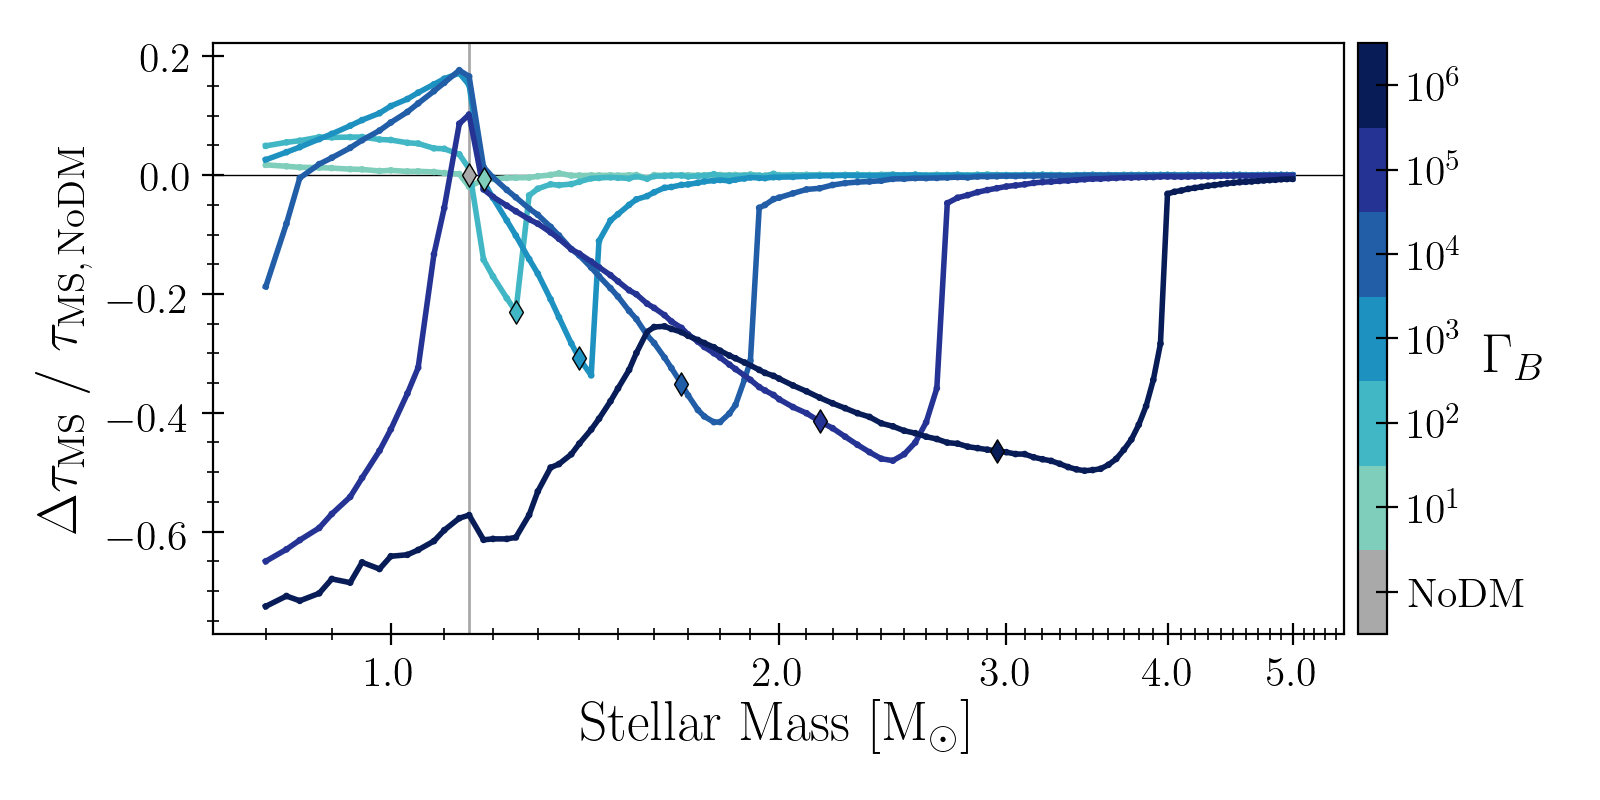
\includegraphics[width=\textwidth]{plots/mstau.png}
    \caption{CHANGES: yaxis label remove 'MS', don't italicize 'NoDM'. xaxis label -> Star Mass, values -> 1,2,.. need more tick marks. Colorbar rotate gammaB to face up. \arz{x-axis should be logarithmically spaced, but we don't want the "$\times 10^0$" on the labels.}
    Change in MS lifetime relative to NoDM model. The presence of DM generally shortens the MS lifetime.
    Differences in the two categories of stars in this mass range can be seen here in the non-monotonicity around roughly 1.3 Msun.
    }
    \label{fig:mstau}
  \end{figure*}

  % Teff plot
  \begin{figure*}
    \centering
    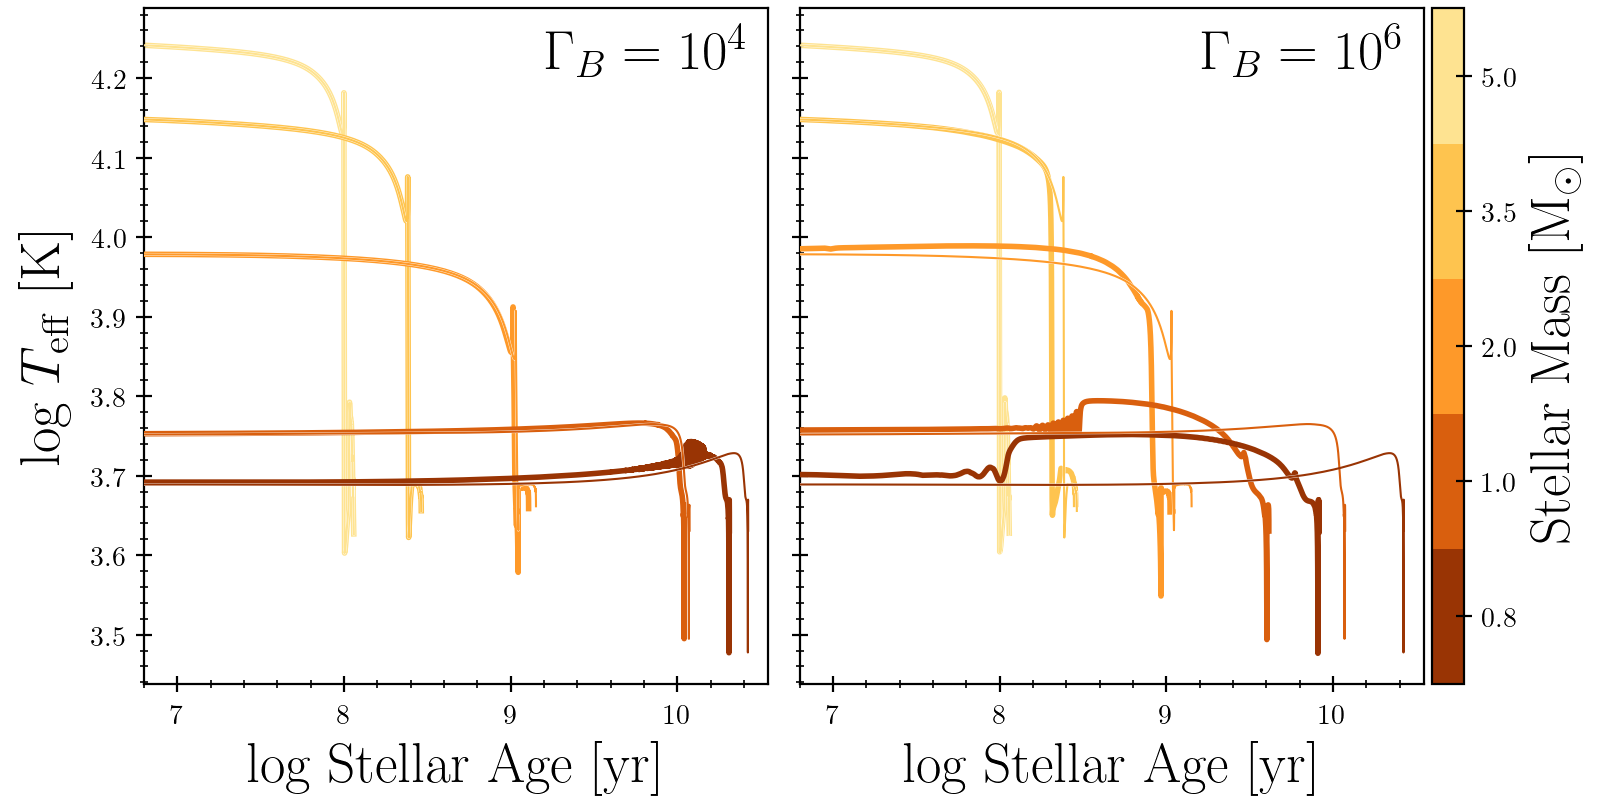
\includegraphics[width=\textwidth]{plots/Teff.png}
    \caption{CHANGES: increase all font sizes. yaxis label Teff italicized / K. xaxis lower limit 7. Perhaps remove c4 panel and make the 3rd panel a zoom-in that includes c4?}
    \label{fig:Teff}
  \end{figure*}

  % stellar tracks plots
  \begin{figure*}
    \centering
    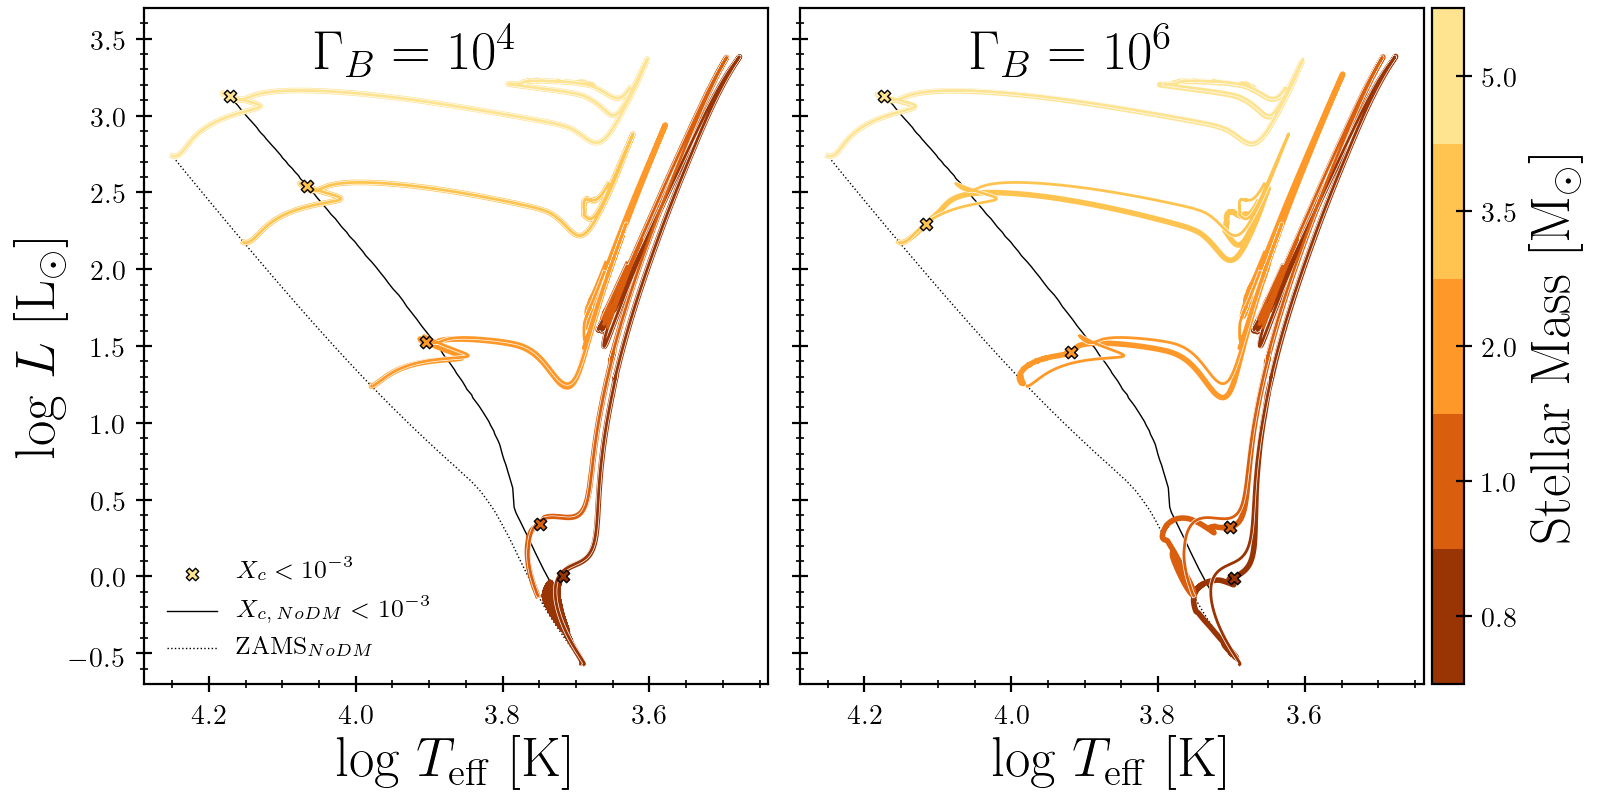
\includegraphics[width=\textwidth]{plots/tracks.png}
    \caption{CHANGES: all font sizes bigger except plot labels. axis labels log(variable (italic)/ unit). Add and label ZAMS line.}
    \label{fig:tracks}

  \end{figure*}

  % isochrones plots
  \begin{figure*}
    \centering
    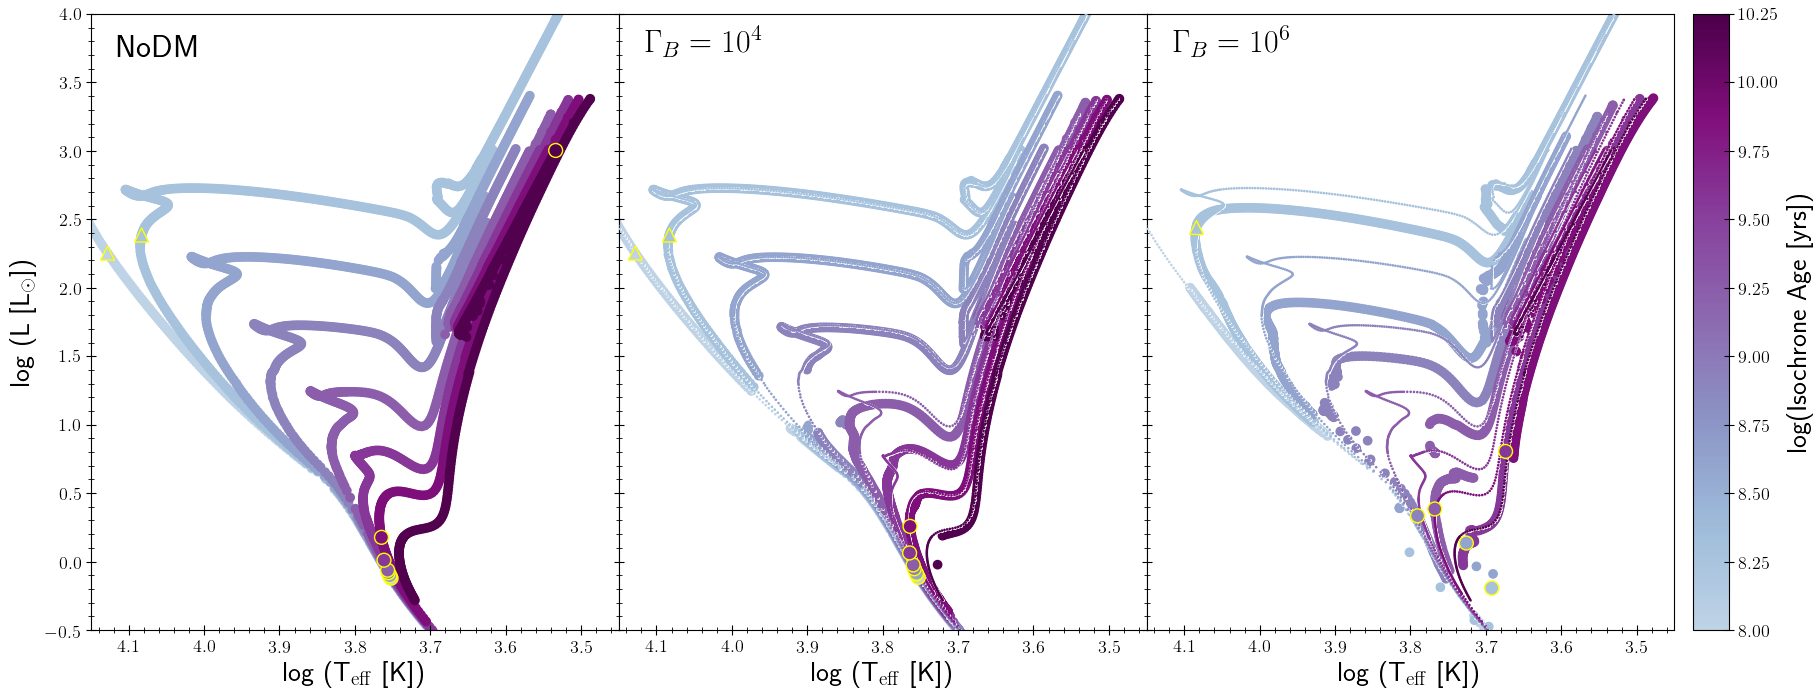
\includegraphics[width=\textwidth]{plots/isos_cb.png}
    \caption{CHANGES: all font sizes bigger except plot labels. axis and colorbar labels log(variable (italic)/ unit). Consider zoom in of lower right on c6 plot. Triangles are 3.5$\Msun$, circles are 1.0$\Msun$. There is missing data where the isochrone code did not interpolate. This is due to non-monotonicity in the initial mass - age relation of a given EEP (equivalent evolutionary phase), which is a known problem that Dotter discusses in his paper.}
    \label{fig:isos_cb}
  \end{figure*}


  \todo{still need to re-write this paragraph.} We find that, for stars significantly affected by ADM energy transport, the general effect is to shorten MS lifetimes (see Figure \ref{fig:mstau}) so that, for a stellar populations of a given age, the MS turn-off happens at a lower mass and the stars evolve through the sub-giant branch at a lower luminosity (see Figure \ref{fig:isos}) when ADM cooling is operative. This causes isochrones of clusters in high $\gb$ environments to appear older than their standard model counterparts. This becomes noticeable in the highest $\gb$ environments around 0.2 Gyr as stars with $\rm{M} \approx 4 \Msun$ begin to leave the MS. Prior to this the stars have not had enough time to capture a sufficient number of WIMPs for ADM-driven energy transport to be a significant contribution to the overall energy transfer within the star.

  \arz{In what follows, an important change will be that we should discuss the figures in the order in which they appear.
  This is very standard practice and I don't think we should deviate from that.}

  \arz{For this first paragraph, I might attempt to do something like the following. I think this
  gives a nice introduction to the basic result, incorporates what the reader needs to know about
  low-and high-mass stars (so we can remove that part from the introduction), and segues into
  the separate subsections about low- and high-mass stars. This may need some editing, but I hope
  you get the idea.}
  In general, we find that ADM within stars alters stellar MS lifetimes and post-MS evolution. The alteration
  of MS lifetimes is shown in Figure~\ref{fig:mstau}. For the purposes of this figure, we have defined the
  MS to end when the core abundance of hydrogen falls below XXXXX. In Fig.~\ref{fig:mstau},
  it is apparent that in most, but not all, scenarios that we study, MS lifetimes are reduced due to ADM.
  Examining Fig.~\ref{fig:mstau} more closely, stellar lifetimes relative to the standard case with no
  ADM increase from low masses until they turn over and decrease again. The mass at which this decrease
  occurs varies based upon the environmental boost factor $\gb$, which is a proxy for the strength of the
  cooling effect. However, the reason for the turnover is related to a fundamental distinction between
  low-mass stars and high-mass stars.

  \arz{Maybe you want to add a discussion of Figure~2 right here as well?}

  To understand this feature better, consider standard stellar evolution in which there is no influence from
  dark matter of any kind. In this case, stars burn hydrogen to produce helium through two channelsl, namely
  the proton-proton (pp) chain and the carbon-nitrogen-oxygen (CNO) cycle
  \arz{Cite one or more standard references on stellar structure here. I am partially
  to Kippenhahn, but whatever you like is fine.}. The pp chain dominates energy
  production in stars with core temperatures $\Tc \lesssim 2 \times 10^7 \mathrm{K}$ and the
  rate of burning scales with temperature very roughly as $\epspp \propto T^4$. The CNO
  cycle dominates nuclear burning in stars with higher core temperatures and CNO burning rates scale
  much more strongly with temperature: $\epsCNO \propto T^{16-20}$. The core temperature
  that separates the CNO cycle from the pp chain corresponds to a stellar mass of approximately
  $\Mstar \approx 1.3 \Msun$. This distinction in burning rates corresponds to a fundamental
  difference in stellar structure. In pp-dominated stars with $\Mstar \lesssim 1.3 \Msun$,
  the transport of energy from the core burning region
  is dominated by photon diffusion. Energy transport in the cores of such stars
  is said to be radiative. In CNO-dominated stars with $\Mstar \gtrsim 1.3 \Msun$,
  radiative energy transport is insufficient to carry away the energy produced by hydrogen burning.
  Consequently, these high-mass stars have convective cores. In what follows, we will consider
  results for high-mass stars and low-mass stars separately and we will demonstrate that ADM
  has distinct effects on the evolution of low- and high-mass stars.

\subsection{High-Mass Stars: \mrangehigh}
\label{sub:highmass}

  % 3.5Msun, energy and convection
  \begin{figure*}
    \centering
    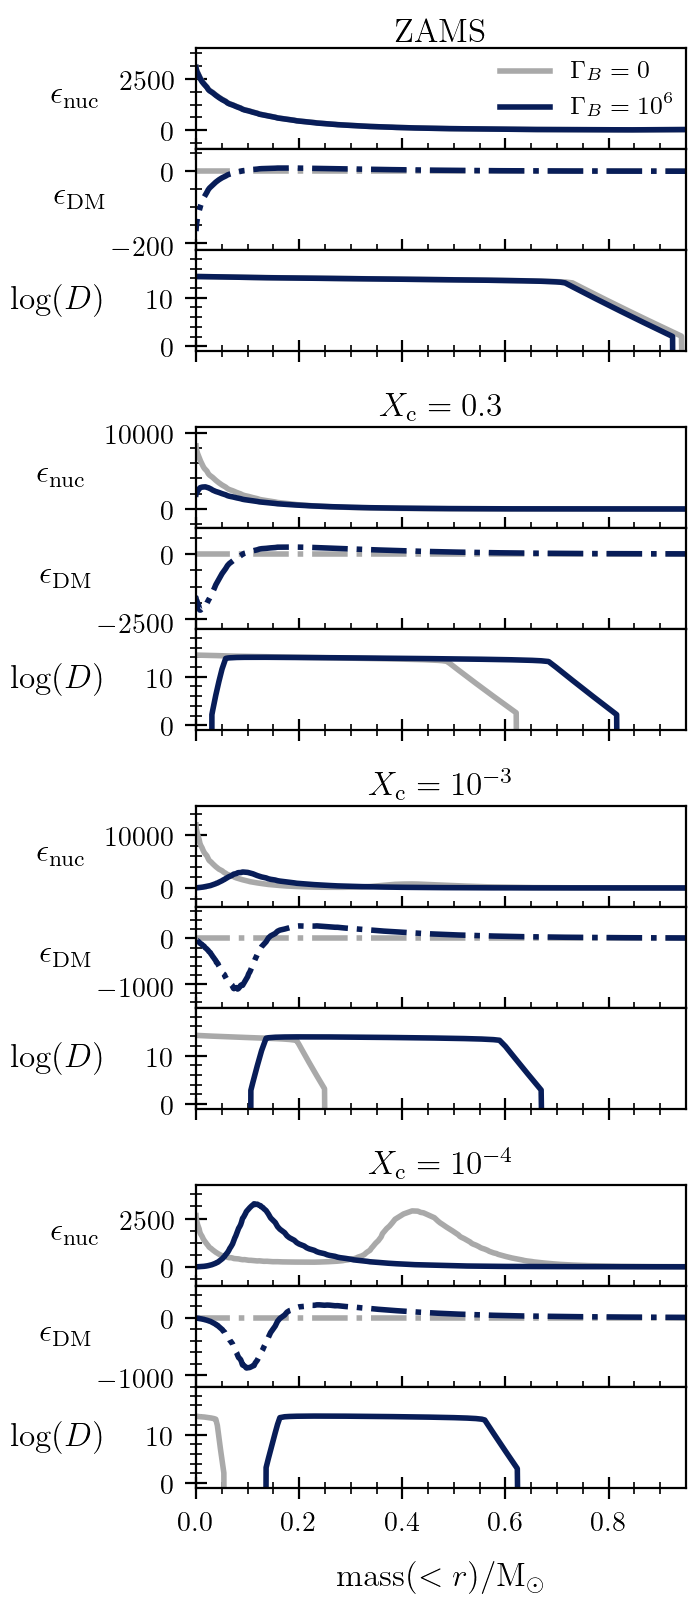
\includegraphics[width=\textwidth]{plots/m3p5.png}
    \caption{
    CHANGES: main title ''. column titles 'energy production and transport', 'convection'. yaxes label with units, remove them from legend. put 0 line on epschi for c0. fix the scale? xaxis label m(<r)/Msun. reduce linewidth. increase space between rows, maybe decrease height of plots.
    CAPTION: 3.5Msun. Cboost colors are the same as the previous plots. Time moves down the page. Left column (note large scale changes): eps nuc is on the left axis, DM energy transport is on the right. Negative (positive) values of epschi indicate DM is removing (depositing) energy. Right column: convective mixing (log(D) where D is diffusion coefficients of convection + overshoot.). As the radiative core grows in the c6 model, the burning gradually shifts outward to shell burning, following the inner edge of the convective shell. The hydrogen supply is not replenished outside the convective zone. NOTES: I'll put the grey arrows in exactly the right place once we settle on which time steps to show. The $h1_c$ legend is just a check to make sure the specific profile used is close enough to the one I wanted. I will remove this for the final plot.}
    \label{fig:m3p5}
  \end{figure*}

  In standard models, MS stars with $\Mstar \gtrsim 1.3 \Msun$ are powered primarily by the CNO cycle.
  This has several important consequences:
  (1) the burning rate is much higher than in pp-dominated stars;
  (2) the burning rate is extremely sensitive to core temperature;
  and (3) stellar cores must be convective in order to carry away the
  energy produced by core hydrogen burning.
  Central convection typically extends beyond the burning region,
  giving the star a source of new nuclear fuel as hydrogen from outside of the
  core is mixed into the stellar center.
  \arz{A better way to say this that may eliminate the need for any
  footnote might be to say something along the lines of "This influx of unburnt hydrogen into
  the stellar core extends the MS lifetime of the star beyond what it would have been had
  there been no convection.}
  As a result, convection extends the MS lifetimes
  \footnote{This extension is subdominant. Central temperatures increase with stellar mass, causing the burning rates to increase dramatically which shortens standard model stellar lifetimes so they decrease approximately as $\tau \propto \Mstar^{-2.5}$.}.
  Once hydrogen throughout the convective zone is depleted, the star exits the MS.
  At this point, the burning rate rapidly decreases and
  the star loses more energy at its surface than is being generated by burning.
  Gravity temporarily dominates and the star contracts until the
  internal temperature increase is sufficient to ignite hydrogen in a shell
  outside the depleted core.
  This can be seen in the `NoDM' models (light blue \qus{green? yellow?} \arz{light blue})
  in Figure~\ref{fig:m3p5}. \arz{Tell the reader how they see this effect. What is the reader looking for?}
  \qus{why does the convective region shrink while burning rate increases?}
  The contraction causes a temporary increase in
  $\Teff$ and a feature in the star's HR diagram called the convective hook (see Figures \ref{fig:tracks} and \ref{fig:isos_cb}).
  See \citet{Pols1990StellarEvolution} for more details.
  \arz{If you want to discuss Figure~5 prior to discussing the isochrones,
  then we should switch the order in which the
  figures appear in the paper. Figure~5 will
  need a detailed caption and/or a more detailed description
  in the main text of the paper.}


  If a star captures enough ADM, the combination of dark matter + radiative energy transport becomes sufficient to carry the flux from nuclear burning. Convection disappears from the center first (where ADM energy transport is most efficient) and retreats away from the core, into a narrowing shell. Without convective mixing, the central hydrogen supply depletes and so the burning also shifts into a shell, following the lower boundary of the convective zone (Figure \ref{fig:m3p5}). The result is that these stars leave the MS earlier and at a lower luminosity, and they skip the convective hook altogether (Figure \ref{fig:tracks}). This makes the isochrones appear older than their `NoDM' counterparts (Figure \ref{fig:isos_cb}). The effects disappear as $\Mstar$ approaches $5 \Msun$ because stellar lifetimes become too short for a sufficient amount of ADM to build up.


\subsection{Low-Mass Stars: \mrangelow}
\label{sub:lowmass}

  % 1.0Msun, energy and temperature
  \begin{figure*}
    \centering
    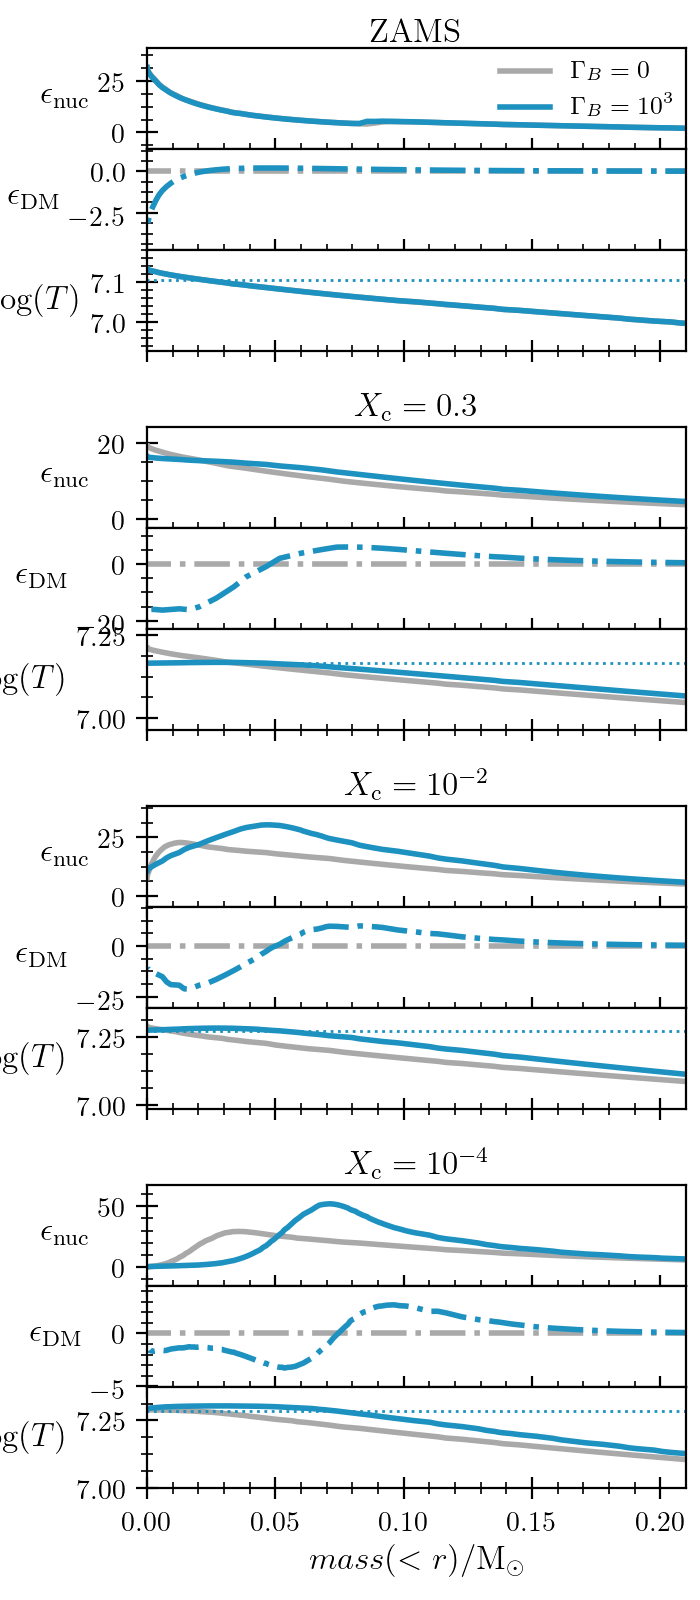
\includegraphics[width=\textwidth]{plots/m1p0c3.png}
    \caption{1.0Msun. Cboost colors are the same as the previous plots. Time moves down the page. Left column: (same as previous plot) eps nuc is on the left axis, DM energy transport is on the right (note large scale changes here). Right column: temperature (DM temperature marked as thin dotted line.
    DM energy transport decreases the burning in the core and pushes the burning into a shell more quickly than the reference models.
    }
    \label{fig:m1p0_a}
  \end{figure*}

  % 1.0Msun, energy, temperature, density profiles
  \begin{figure*}
    \centering
    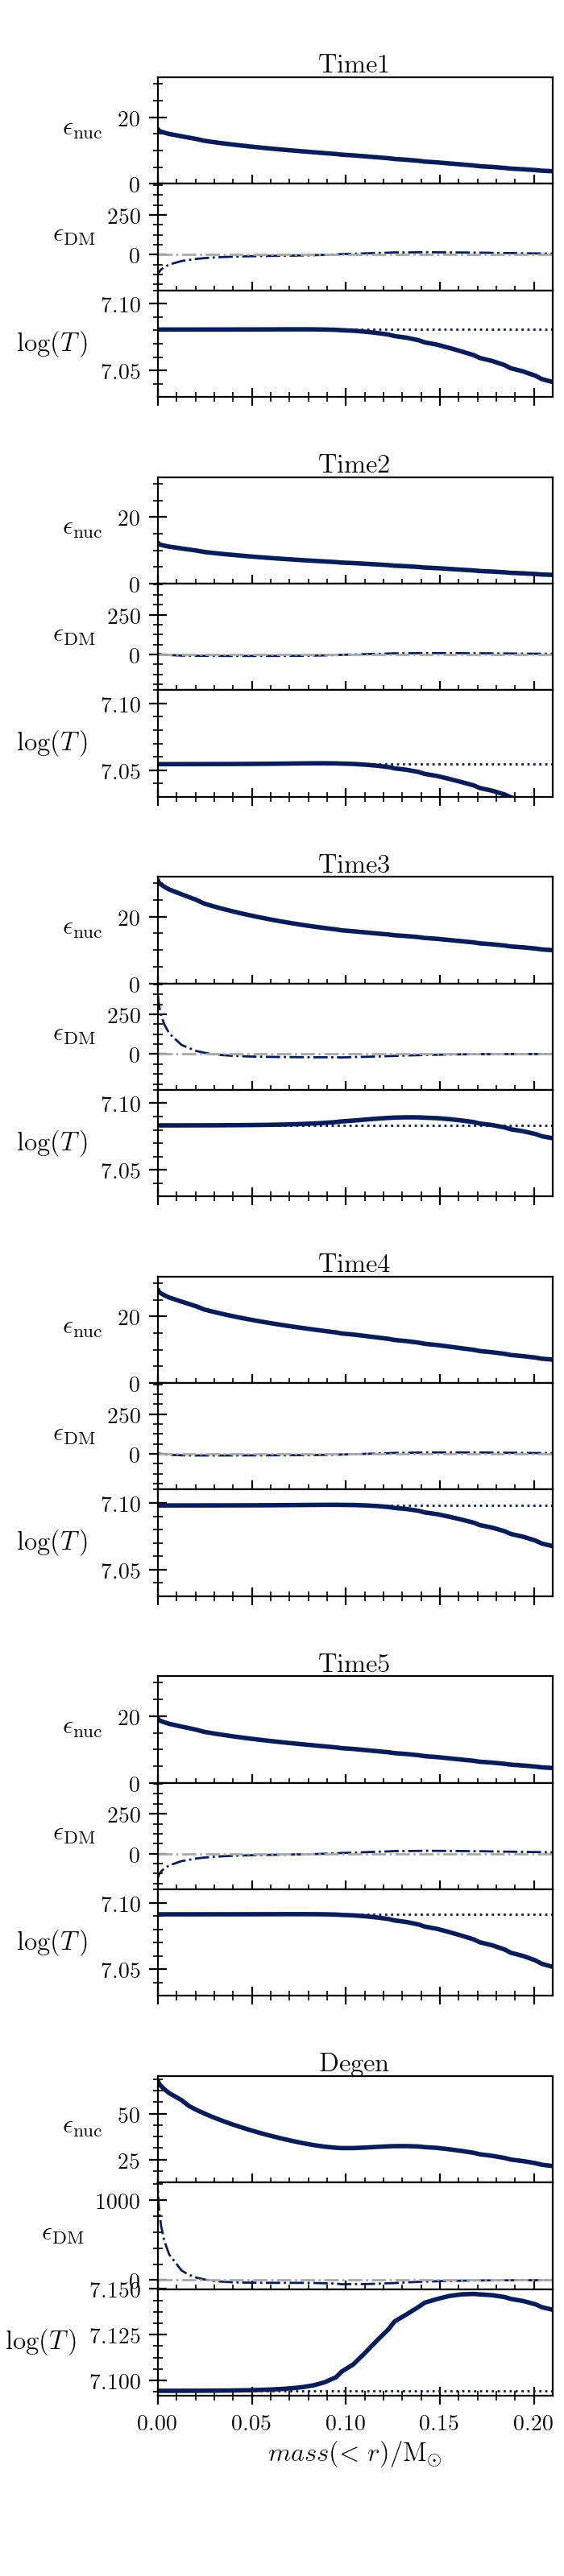
\includegraphics[width=\textwidth]{plots/m1p0c6.png}
    \caption{Star mass 1.0Msun, $\Gamma_B = 10^6$ (colors are different than previous plots). Time moves down the page with rows correspond to times from figure \ref{fig:m1p0_kipp}. 'Time1-5' were chosen to show the progression and extremes of DM energy transport during one oscillation cycle. Scales are fixed for ease of comparison. 'Degen' shows conditions after the oscillations stop, when electron degeneracy pressure is supporting the core (note scale changes). Left column has $\epsilon_{nuc}$ on left axis (red) and DM energy transport on the right (blue). Right column has logT on left axis (red, with T$_x$ marked with thin dotted line) and logRho on the right axis (blue).
    %   Time 1: 3.1736e8 yrs, xheat$_c$ is maximum, T$_c$ and $\epsilon_c$ are increasing. Time 2: 3.229e8 yrs, xheat$_c$ is minimum, T$_c$ and $\epsilon_c$ are decreasing (this should be first time shown in plot). Time 3: 3.288e8 yrs, T$_c$ is minimum, xheat$_c$ and $\epsilon_c$ are increasing. Time 4: 3.81e8 yrs, core degeneracy has become significant.
    }
    \label{fig:m1p0_profs}
  \end{figure*}

  % 1.0Msun c6 Kippenhahn with profile times labeled
  \begin{figure*}
    \centering
    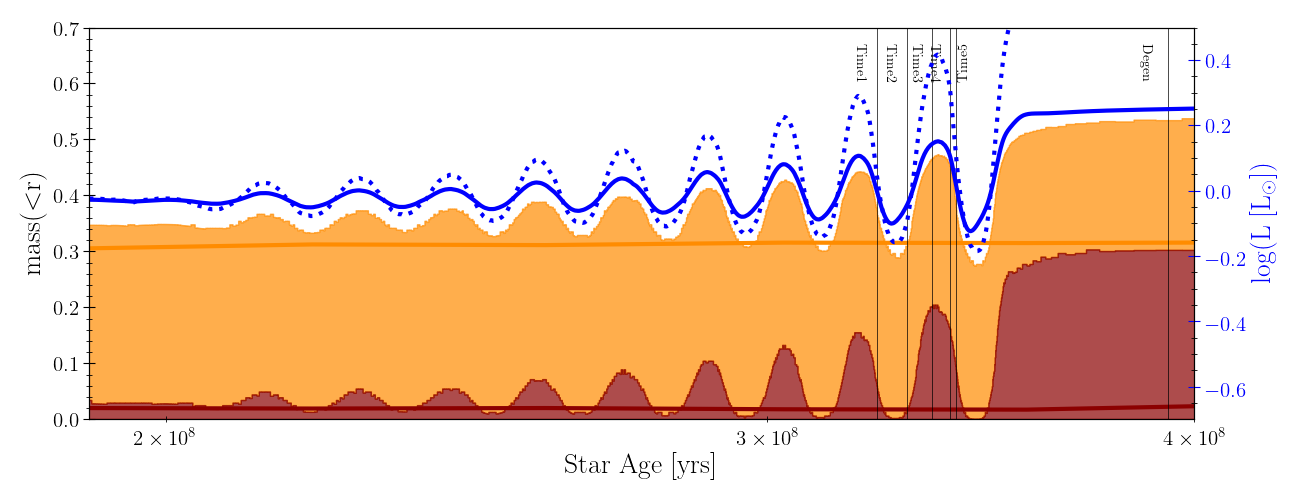
\includegraphics[width=\textwidth]{plots/m1p0c6_age.png}
    \caption{Star mass 1.0Msun, $\Gamma_B = 10^6$.  Figure \ref{fig:m1p0_profs} shows profiles of the star at the times marked here by vertical black lines.
    % Star mass 1.0Msun, c6, xaxis is age. Top plot shows core burning volume (red shaded area, left axis. Add color variations to show intensity) and L (right axis. Important lines are in the middle, red (log L) and white (log LH). Top and bottom lines should be removed from plot.
    Yellow and red show burning intensity as a function of age and mass coordinate (left axis) (I believe the burning thresholds are 1 erg/g/s and 10 erg/g/s respectively, but I'm a little confused about the mesa output and I need to check with Héctor or Carles.) Darker yellow and red lines mark the burning extent of the NoDM model over this time period.
    Blue line is luminosity (right axis). NOTE: Dotted blue line is hydrogen burning luminosity (I will probably remove this line for the final plot, but I want to check with Carles to make sure the behavior makes sense. I think the explanation is: When LH>L star is producing more energy than it is losing, causing it to expand, and . I have a separate plot of the radius that we can look at if needed. Actually could add logR to this plot.)
    %   (bottom plot). Bottom plot shows R$_{\star}$ (yellow, left axis) and r(m<0.01). As the core contracts, the envelope expands.
    }
    \label{fig:m1p0_kipp}
  \end{figure*}

  Standard model stars in this mass range have relatively low central temperatures and so are powered primarily by the pp-chain, which is much less sensitive to the temperature. This means the burning does not peak as strongly at the center and radiative transport is sufficient to carry the energy flux, so the core is not convective. Without convective mixing, hydrogen depletes first at the very center and the burning shifts outward gradually, avoiding the instability that causes the convective hook in standard CNO-powered stars. This behavior is very similar to high-mass stars that collect large amounts of ADM, which contributes to isochrones appearing older as $\gb$ gets large.

  Since the burning rate is much lower, the same number of captured dark matter particles have a larger effect in this mass range. As stars with $\gb$ as low as $10^2$ \todo{check this number for several masses} enter the MS, ADM is already transporting a significant amount of energy away from the center ($\epsx \approx \epspp$ near $r=0$) and depositing it in a shell at $m(<r) \approx 0.1 \Msun$. This causes the temperature, and therefore the burning rate, to be lower at the center and higher in a shell relative to standard models. Stars in environments with $\gb \lesssim 10^4$ are able to remain stable in this configuration. See Figure \ref{fig:m1p0_a}.
  % and their evolution is not significantly altered \tjr{looks significant in MStau plot...?}.

  Models with $\gb \gtrsim 10^4$ capture enough ADM so that $\epsx \gg \epspp$ near $r=0$ which destabilizes the core and sets up a series of oscillations. \todo{check different masses, particularly 0.8Msun for which the effect may extend down to c4.}
  (see Figure \ref{fig:m1p0_profs} Time 2, left plot). As $\Tc$ continues to decrease, the temperature profile inverts and the center is no longer the hottest region in the star. Eventually, $\Tc < \Tx$ and dark matter begins moving energy back towards the center ($\epsx(r=0) > 0$, see Time 3 in Figure \ref{fig:m1p0_profs} \todo{possibly pick this time a little later, after xheat at center >0}). This increases both the central temperature and burning rate until $\Tc > \Tx$ and the cycle starts over. The effects propagate out to the surface where
  $L$, $\Teff$, and $\Rstar$ all oscillate in response to changes in the core. Similar oscillatory behavior was noted in \citet{Iocco2012} \qus{seems like I need to say more here, but I'm not sure what. The Iocco paper (arXiv:1201.5387v1) states the following: "In spite of our efforts, we have not been able to fully understand the reason of the oscillations seen in Figure 3, whether they are a physical effect arising from the “bouncing” of the central temperature on the WIMP temperature floor, or a numerical artifact. We have however checked that the existence of oscillations does not affect our results nor does change our conclusions. Beside the theoretical consistency of the intepretation presented in the paper, one can be convinced of the actual physical consistency of our results with observations based on several numerical experiments we have performed: ..."}.

  The process repeats, with increasing amplitude, until the central temperature falls low enough that the core becomes significantly degenerate. Once electron degeneracy pressure can support the core, the temperature decouples from the equation of state and the star quickly settles into a more stable configuration with a significant temperature inversion (see Time 4 in Figures \ref{fig:m1p0_profs} and \ref{fig:m1p0_kipp}).

  Overall, the ADM captured by these stars causes burning in a larger volume and at a higher rate than in standard models (see Figure \ref{fig:m1p0_kipp}). The stars then burn through the central hydrogen supply faster and leave the MS earlier: by 2.5 Gyr, solar mass stars with $\gbpow{6}$ have already left the MS and are climbing the red-giant branch. Note that the 2.5 Gyr, $\gbpow{6}$ isochrone is most similar the 10 Gyr, NoDM isochrone (Figure \ref{fig:isos_cb}).


  Notes:
  hydrogen depletes in shell first.
  % \tjr{I'm not totally sure this is the CAUSE of the oscillations, but I've checked a lot of other things and ruled them out. Lower cboost models sometimes transport more energy than produced by burning, but never more than a few erg/g/s. c5 and c6 models transport a minimum of ~5 erg/g/s more than is generated from burning and usually much more than that (a few hundred erg/g/s during oscillations, up to 1000 erg/g/s by the time it goes degenerate).}

  % \tjr{burning changes before temperature which I don't really understand. See figure \ref{fig:osc_scaled_values} for more info. Order of changes seems to be: extra heat -> density -> burning -> temperature. Tried to check how mesa calculates the burning rate to find dependencies other than temperature, but the calculation seems pretty scattered and complicated and I couldn't find anything useful.}

  Possible work for future: 1. vary DM mass and cross section (given observational constraints) to see how quick the effects vanish. 2. model iso curves and quantify how much older they look.


  %--------------------


  %--------------------
  % % m1p0 c0 kipp
  % \begin{figure*}
  % \centering
  %   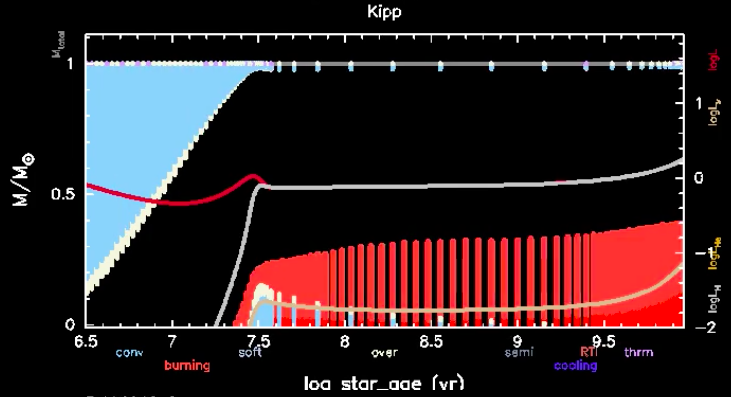
\includegraphics[width=\textwidth]{plots/m1p0c0_kipp.png}
  %   \caption{\label{fig:m1p0c0_kipp}Star mass 1.0Msun, c0, Main sequence burning. Note that the burning (shaded in red, left axis) doesn't extend as far as c6 model.}
  % \end{figure*}
  %--------------------

  %  \tjr{why are they destabilized? centerRho is higher, centerT is lower, Tmax-Tc is lower than lower cboosts (except extreme oscillations), oscillations start before Tc-Tx<0. what makes it go from transporting energy away from center to transporting to center? temp profile flattens (inverts? but cb<5 also invert so why are they still stable? they transport more energy than epsnuc. yes, oscillations turn on more slowly in c5, stable at $\epsilon_{\rm{x}}(r=0) \approx \epsilon_{\rm{nuc}}(r=0)$ for beginning of MS)}

  % The PP chain is less efficient? NO! PP, CNO have same net energy per pp fusion.

  % Nx and nxcenter are higher here than high mass stars, but wimps transport less heat here. why? Tx-Tc is much lower. but they still have a larger effect than in high mass stars because there is less energy flux to carry.

  % --------
  % 1.0 pgstar notes:
  % what i think is happening:
  % temp is lower so burning rate is much lower.
  % wimps take kinetic energy from protons. transport all of the energy generated from burning plus additional kinetic energy. burning rate goes down. temperature goes down.
  % temp and burning rate are still high (higher than c0?) in a shell where wimps have been depositing the energy. temp inverts and wimps start moving energy back to core (largest deltaT just before this happens?). proton kinetic energy goes up (so they are more likely to fuse when colliding) and burning rate goes up (largest deltaT here? no.).
  % 2 energy sources increase so temp goes up. temp no longer sufficiently inverted, wimps start moving energy away from core and process starts over.

  % stabalizes with large T inversion (deltaT=7.13-7.19 =4e-2) when degeneracy becomes important.

  % at center unless otherwise specified:
  % General oscillation pattern:
  % xheat negative and decreasing
  % burning, temp, and R decreasing, deltaT O(5e-4)
  % xheat peaks low, stays close for awhile

  % at 58 secs:
  % xheat, burning, temp all decreasing
  % TMR increasing, R decreasing

  % xheat peaks low at -80 (deltaT=7.0660-7.0656= 4e-4) then goes up
  % burning peaks low at 11 (TMR peaks high at same time or slightly before) then goes up
  % T peaks low at 7.0567 (deltaT=7.0573-7.0567 =6e-4) then goes up

  % xheat increases past 0 (deltaT=7.0582-7.0576= 6e-4)
  % luminosity goes negative at 0.08Msun
  % deltaT increasing

  % xheat peaks at 130 (deltaT=7.0711-7.0695= 16e-4) then oscillates up and down a bit
  % after last xheat peak, burning peaks at 20 then goes down
  % deltaT decreasing

  % xheat decreases past 0 (deltaT=7.0777-7.0771 =6e-4)
  % T peaks at 7.0772 (deltaT=7.0777-7.0772 =5e-4) then goes down
  % luminosity to zero (non-negative)

  % xheat peaks low at -100 (deltaT=7.0725-7.0722 =3e-4) then oscillates up and down a bit
  % after last xheat peak, burning peaks low at 11 then goes up
  % T peaks low at 7.0553 (deltaT=7.0558-7.0553 =5e-4)

  % xheat increases past 0 (deltaT=7.0569-7.0562 =7e-4)
  % luminosity goes negative at 0.08Msun

  % earlier:
  % xheat, burning, temp all decreasing
  % xheat peaks low at -40 then goes up
  % burning peaks low at 12 then goes up
  % T peaks low at 7.0592 then goes up

  % burning peaks at 14.5
  % xheat crosses 0, decreasing
  % T peaks high at 7.0664
  % burning decreasing
  % temp decreasing

  % temp is inverted
  % burning increasing
  % xheat positive
  % core radius is shrinking
  % R increasing

  % center temp increases, still inverted
  % xheat positive and decreasing
  % burning peaks
  % xheat goes negative
  % burning decreases

  % 1.0 pgstar notes end
  % --------


  % Stars leave the main sequence at a lower luminosity, which continues through the sub-giant branch (since He core mass is lower?), and the convective hook disappears. Caused by: lower gradT => lower central burning (CNO temp dependence) => core convection turns off => transition to H shell burning is more gradual.


\section{Discussion and Conclusions}
\label{sec:conclusions}

  \arz{I think that most of your conclusions section could be (1) a summary of our results and (2) speculations on how to turn this into a constraint in the future.}

\section*{Acknowledgements}



%%%%%%%%%%%%%%%%%%%%%%%%%%%%%%%%%%%%%%%%%%%%%%%%%%







%%%%%%%%%%%%%%%%%%%% REFERENCES %%%%%%%%%%%%%%%%%%

% The best way to enter references is to use BibTeX:

\bibliographystyle{mnras}
\bibliography{references}

%%%%%%%%%%%%%%%%%%%%%%%%%%%%%%%%%%%%%%%%%%%%%%%%%%

%%%%%%%%%%%%%%%%% APPENDICES %%%%%%%%%%%%%%%%%%%%%

% \appendix

% \section{section}
% \label{sec:sec}



%%%%%%%%%%%%%%%%%%%%%%%%%%%%%%%%%%%%%%%%%%%%%%%%%%



% Don't change these lines
\bsp	% typesetting comment

\label{lastpage}

\end{document}

% End of mnras_template.tex



Change in main sequence (MS) lifetimes relative to standard model stars with no ADM. Large amounts of ADM (high $\gb$) typically shorten stellar lifetimes. The effect is large at low masses and decreases with increasing stellar mass until $\Mstar \gtrsim 1.3 \Msun$ (where the exact value depends on $\gb$), a result of a change in the fundamental physics between low and high mass stars. The effect then increases with mass until stellar lifetimes are too short to build up a sufficient amount of ADM when the effect abruptly disappears.

The change in MS lifetimes can also be seen in Fig.~\ref{fig:Teff} as the evolution of the effective temperature, $\Teff$.
something's wrong.. 1Msun should live slightly longer than NoDM at $\gbpow{4}$.

The evolution of NoDM models are overplotted as thin lines. Stars undergo a sharp decrease in $\Teff$ as they leave the MS. The time difference between these features at constant mass and different $\gb$ shows the change in MS lifetimes due to ADM. The effect of oscillations discussed in S~\ref{sub:lowmass} can be seen in the $0.8\ \Msun$ ($1.0\ \Msun$) model in both panels (right panel).
CHANGES: right panel, put 1Msun on top?
